%Here is the introduction to the topic.
(here insert an intro paragraphs) 

%The field of High Energy Physics (HEP), also known as elementary particle physics,
%focuses on the study of the fundamental particles that make up the universe and their interactions via the basic forces of nature.
%The quest for the smallest constituent of matter has its route back to the time of ancient Greece;
%however, scientific attempts to understand the smallest constituent of matter started in much more recent time.
%Particle physics emerged as a field of scientific study in the early 20th century,
%when scientists began to probe the subatomic structure of matter.
%Later, developments of high-energy particle accelerators such as the cyclotron and the synchrotron, allowed
%for the study of particles at ever-higher energies and smaller scales.


%next:Standrad model/Quarks/leptpons
\section{The Standrad model}
The standard model (SM) of particle physics is the best theoretical model we currently have that describes all the known fundamental particles and their interactions. Particles in the SM can be classified into two categories based on their spin or Intrinsic Angular Momentum value: fermions have half integer spin while bosons have full integer spin.Fermions particles include particles that make up matter this: electrons, protons and neutrons. All fermions follow Pauli exclusion principle which is essential for building atoms and the periodic table. Fermions can be divided further more into two groups based on the strong force: leptons, do not have strong interactions, and quarks, have strong nuclear interactions. 
 
Quarks cannot be isolated because of the color confinement. They are always found in a bound state known as hadrons interacting via strong force. Hadrons either composed of three quarks, baryons, or a pair of a quark and anti-quark, mesons. Baryons have half integer spin so they are considered fermions while mesons have integer spin so they are considered bosons.

Leptons group consist of three electrically charged particles (electron, muons, tau) and 3 electrically neutral neutrinos that comes in three flavors associated with the electron, muon, tau. The electrically charged leptons interact with all forces except for the strong force while Neutrinos only interact through gravity and weak force

Each group in fermions and leptons can be organized into three generations that only differ in their mass. The heavier generation can decay into the next lighter generation till we reach the lightest one that is stable like (electron, up and  down quarks). “Here insert table that shows these generations”

The force carry particles in the SM are vector bosons with spin 1. The electromagnetic force carried by the photon. The strong force is carried by 8 types of gluons. The weak interaction is carried by two charged W bosons and one neutral Z boson. Higgs boson is a scalar boson with spin 0 that interact with mass.

%%%% draft 1 %%%%%
%The standard model (SM) of particle physics is the best theoretical model we currently have that describes all the known fundamental particles and their interactions.
%Particles in the SM can be clasified into two categories based on their spin or Intrinsic AngularMomentum value: fermions have half integer spin while bosons have full integer spin.                                                  
%Fermions particles include particles that make up matter this: electrons, protons & neutrons. All fermions follow Pauli exclusion principle which is essential for building atoms and the periodic table.
%Fermions can be divided further more into two groups based on the strong force: leptons, do not have strong interactions, and quarks, have strong nuclear interactions.                               
%Quarks are the only the elementary particle that can experience all know forces                                                                                                                         
%In the SM this is strong, weak, electromagnetic forces. There are six flavored quarks: up, down, charm, strange, top and bottom quark. They also have a fractional electric charge
%(up, charm, top) have 2/3 e and (down, strange, bottom) have -1/3 e.
%Quarks cannot be isolated because of the color confinement. They are always found in a bound state known as hadrons interacting via strong force.
%Hadrons either composed of three quarks, baryons, or a pair of a quark and anti-quark, mesons. Baryons have half integer spin so they are considered fermions while mesons have integer spin so they are considered bosons.
%Leptons group consist of three electrically charged particles (electron, muons, tau) and 3 electrically neutral neutrinos that comes in three flavorsassociated with the electron, muon, tau.
%The electrically charged leptons interact with all forces except for the strong force while Neutrinos only interact through gravity and weak force.
%Each group in fermions and leptons can be organized into three generations that only differ in their mass.
%The heavier generation can decay into the next lighter generation till we reach the lightest one that is stable like (electron, up & down quarks). “Here insert table that shows these generations”.
%The force carry particles in the SM are vector bosons with spin 1. The electromagnetic force carried by the photon.
%The strong force is carried by 8 types of gluons. The weak interaction is carried by two charged W bosons and one neutral Z boson. Higgs boson is a scalar boson with spin 0 that interact with mass.
%As of now, the observed fundamental particles and their properties and interactions are thought to be described by the Standard Model (SM) of particle physics.
%The SM includes six quarks (in three generations), six leptons, four gauge bosons, and the scalar Higgs boson along with antimatter particles as shown in Fig.~\ref{fig:SMParticles}.
%%The SM of particle physics successfully describes a vast range of subatomic phenomena with outstanding precision.  ~

\begin{figure}[t!]
\centering
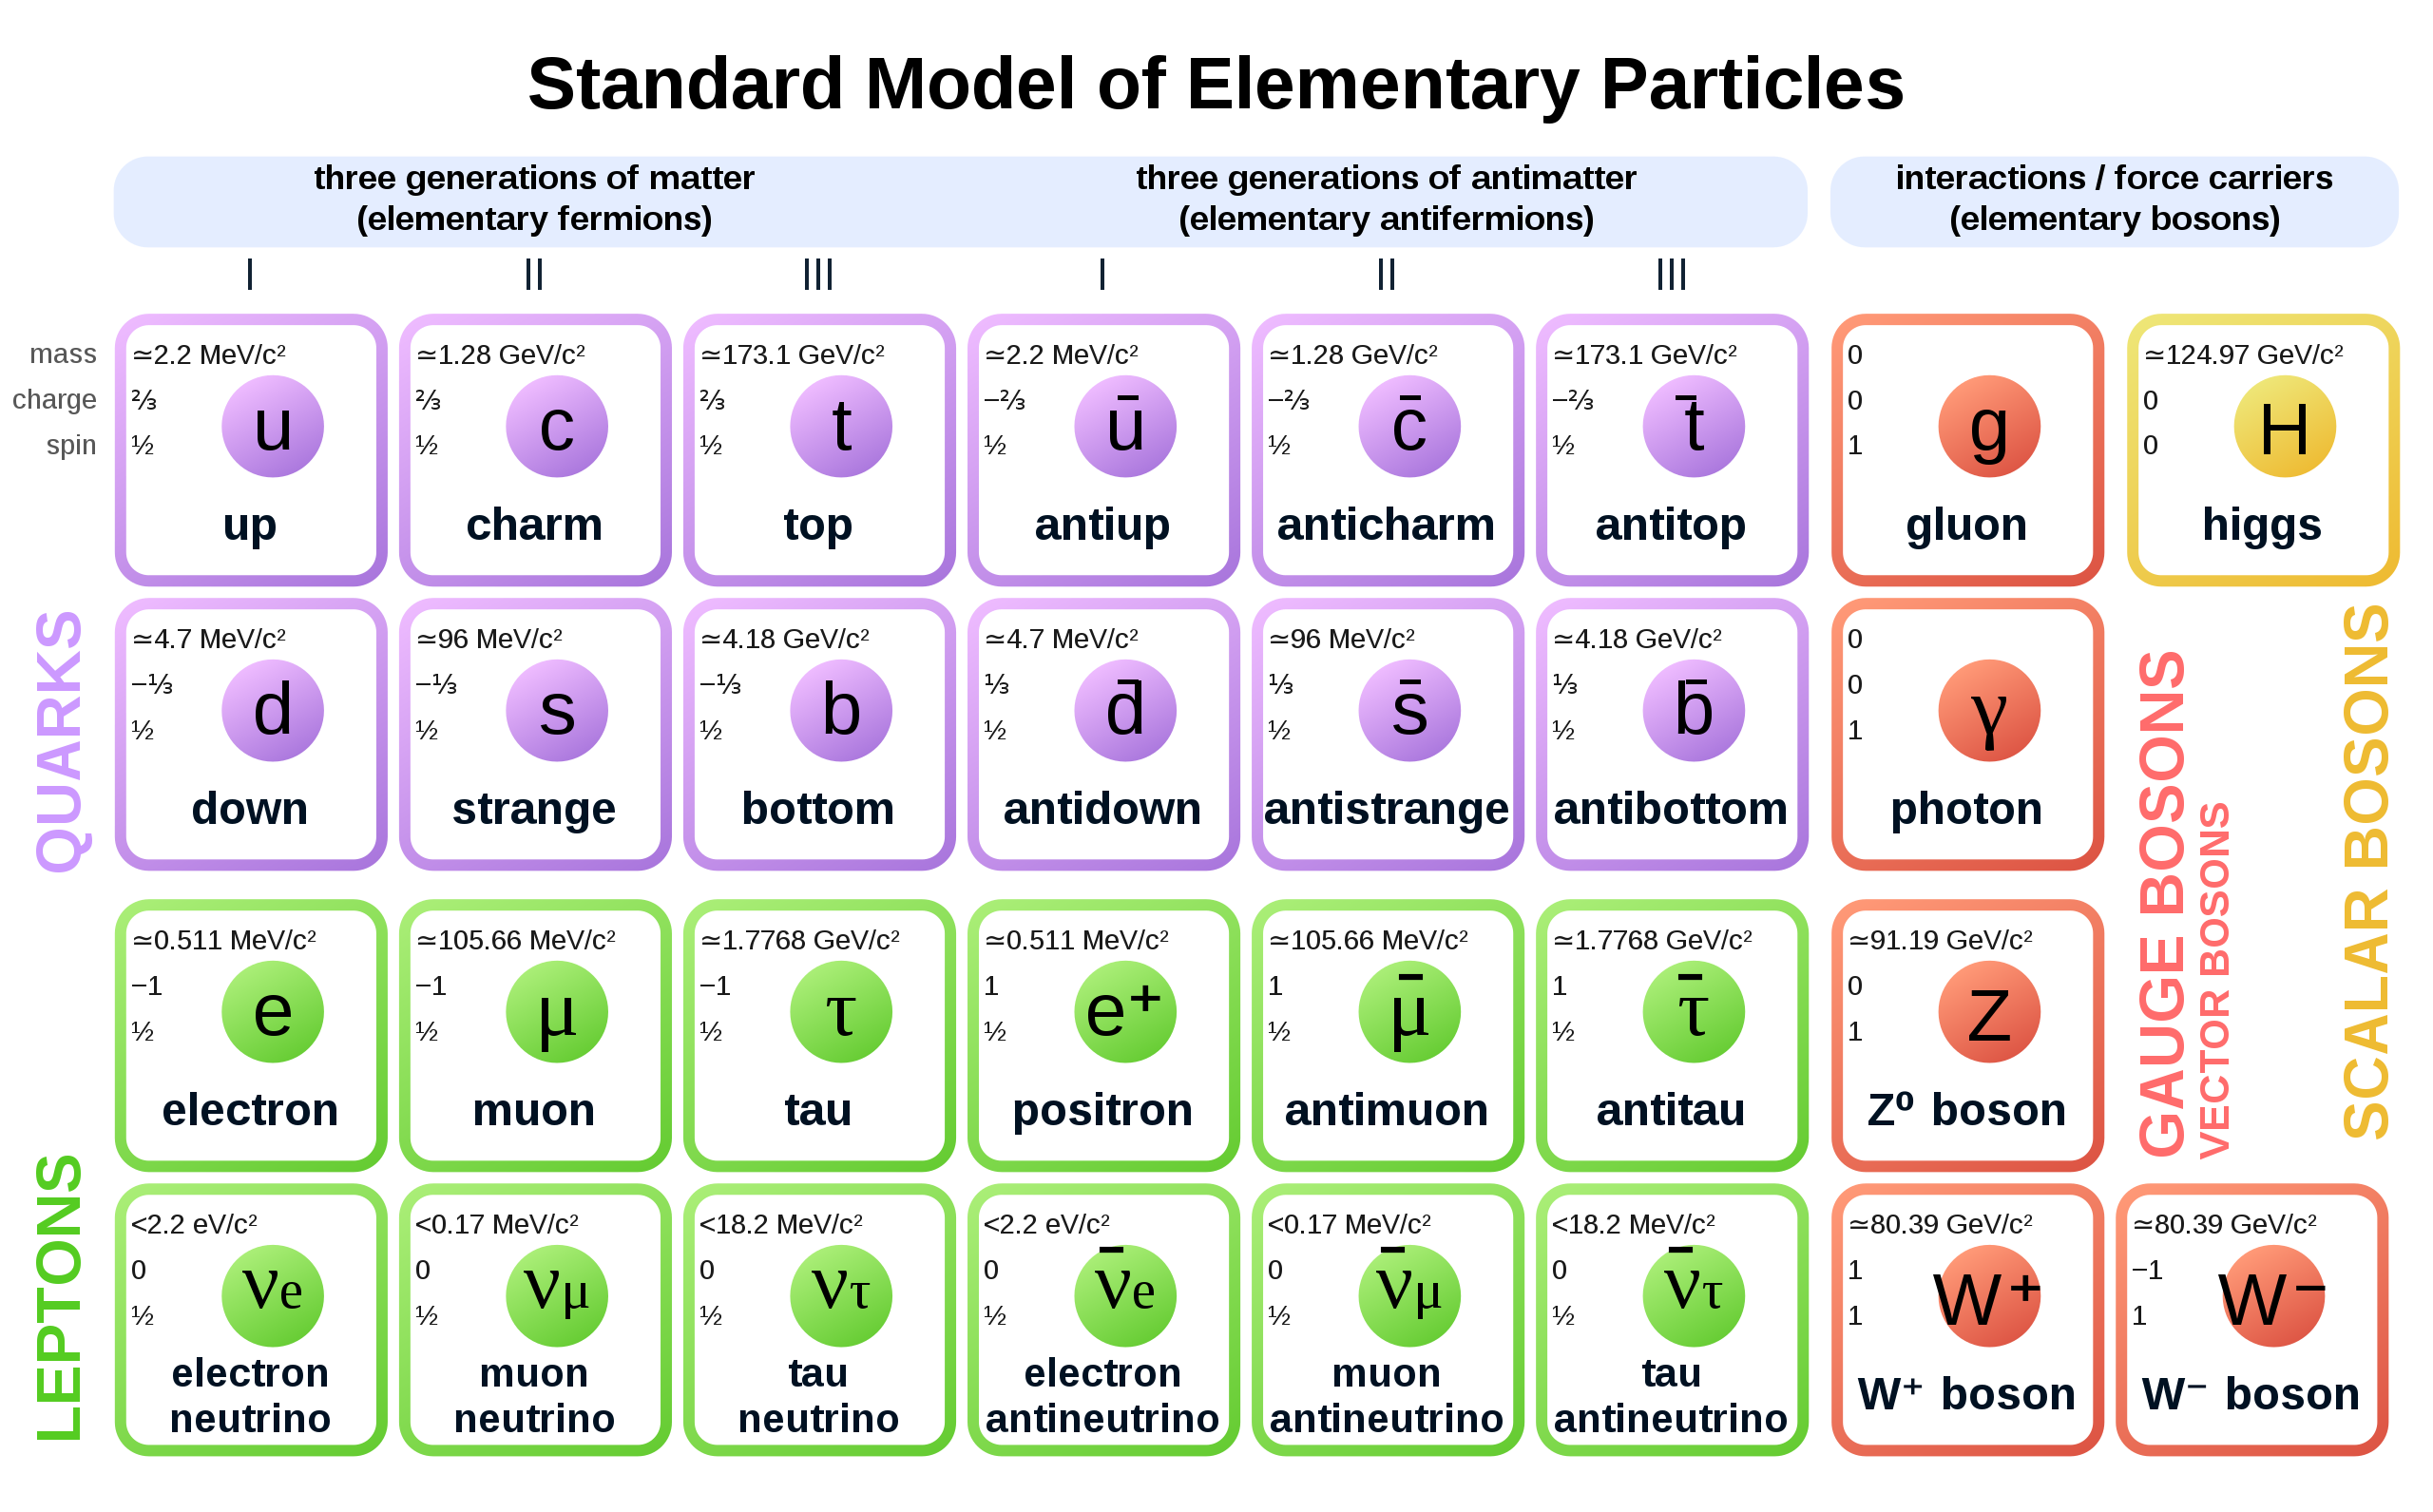
\includegraphics[width=0.99\textwidth]{figures/SMtable.png}
\caption[Summary of standard model fundamental particles]{Summary of SM fundamental particles. Figure source~\cite{SMtable}.
\label{fig:SMParticles}}
\end{figure}

\begin{figure}[t!]
\centering
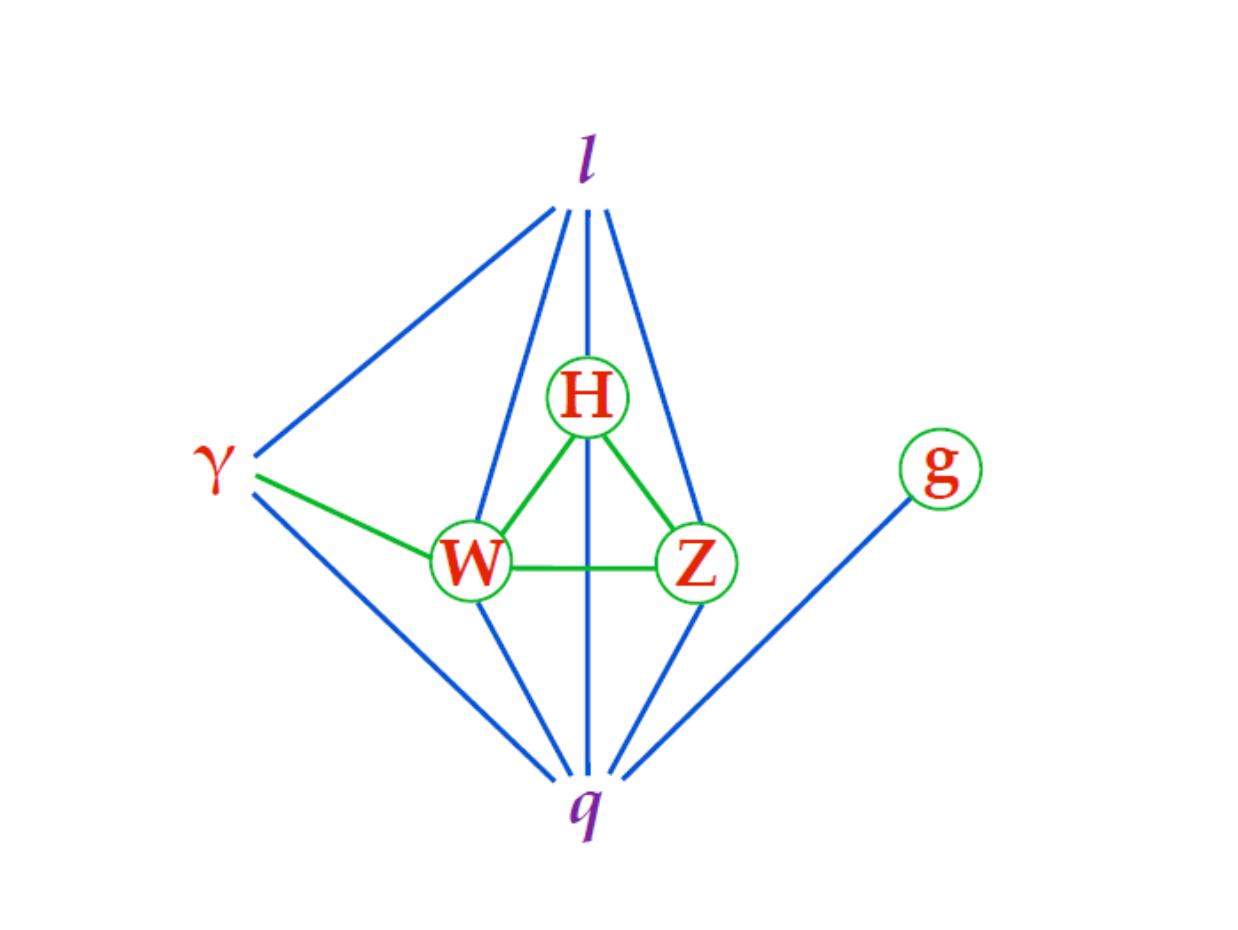
\includegraphics[width=0.99\textwidth]{figures/SM_coupling.png}
\caption[interactions between fundamental particles]{
\label{fig:SMcoupling}}
\end{figure}
%%%%%%%%%%%%%%%%%%%%%%%%%%%%%%%%%%%%%%%%
\section{The large hadron collide}
%\subsection{intro}
The large hadron collider is the most powerful particle accelerator in the world. From its name “Large” refer to its big size which is about 27km in circumference and “Hadron" because it accelerates particles like protons or ions which are known as hadrons.
Lastly, "Collider" because the particles traveling into two beams in opposite directions, are made to collide at four points around LHC ring.  
The LHC is a part of the CERN accelerator complex and sits in a tunnel 100 meters underground at CERN, the European Organization for Nuclear Research, on the border of Switzerland and France near Geneva, Switzerland.   
The CERN accelerator complex is a succession of machines where each machine accelerates a beam of particles to a given energy before injecting the beam into the next machine in the chain. LHC is the last element of this chain where it is designed to collide particles at COM energy up to 14 TeV.
The LHC is made of eight arcs and eight ‘insertions. The arcs contain the dipole ‘bending’ magnets. The layout of the straight section depends on the specific use of the insertion: physics (beam collisions within an experiment), injection, beam dumping or beam cleaning.

%\subsection{Experiments in the LHC}
At the LHC we have 9 experiments: 
ALICE (study heavy ion collisions, QGP) ATLAS, CMS  (general purpose detectors) LHCb (study matter – antimatter asymmetry) ,LHCf (shares intersection with ATLAS),TOTEM (shares intersection with CMS) MoEDAL-MAPP, (shares intersection with LHCb), FASER,SND@LHC.

\subsection{The journey of protons in the LHC}

It all starts from a compressed tank of hydrogen that is connected to source chamber of the linear accelerator.
The Linear accelerator 4 (Linac4) is designed to boost negative hydrogen ions (H with extra electron) to high energies (initial to 1/3 C).
Then the particles are fed to the booster stage. (Proton Synchrotron Booster – PSB).
at the PSB injection point a stripping foil will strip the electrons off the hydrogen anions creating protons that are accumulated as beam bunches in the four PSB rings.
These proton bunches are then recombined at the exit of the PSB and further transferred down theCERN injector chain (accelerated to 91.6 of C).

After that the beam is sent to Proton synchrotron (PS) where the increase of energy does not transfer to velocity.
Instead, it will increase the relativistic mass (accelerated to 99.9 of C).
Then the protons go to the super proton synchrotron. (SPS). Finally, at the LHC has two vacuum pipes where the protons will be going into different directions. 27 km ring of superconducting magnets (keep protons in the ring) that also has accelerating structures (radio frequency cavities) to boost the energy. The LHC’s RF cavities bring the 450 GeV energy of the particles (1 GeV = 1 billion electron volts) to 6.5 TeV source.
The maximum energy is reached in around 20 minutes with the bunches having passed through the RF cavities more than 10 million times.   

There are 4 points where the protons are collided. CMS is one of the them, where this thesis is focus on.  

%%%% draft1 %%%%
% LHC and experiments, Very brief physics summary
%The Hadron Collider at CERN, Geneva, Switzerland is currently the largest and highest energy particle accelerator.
%The LHC consists of a 27-km ring of superconducting magnets with a number of accelerating structures to boost the energy of the particles along the way.
%The LHC can acclerate different types of beams and can produce proton-proton collisions, proton-lead collisions, and lead-lead collisions; however, the main operation mode provides proton-proton collisions.
%The first proton-proton collisions were achieved by the LHC in 2010 at an energy of 3.5 teraelectronvolts (TeV) per beam, about four times the previous world record.
%Over years, the collision energy was inceased and collision rate was also increased.
%As of the year of 2024, the LHC collides protons at the center-of-mass energy of $\sqrt{s}=13.6$\TeV.
%The beams in the LHC cross each other (called bunch crossing) at four points where the ALICE, ATLAS, CMS, and LHCb detectors are located.
%Since the start of its operation, the experiments at the LHC provide a wide range of physics results and advanced our understanding of elementary particles and their interations.
%Among various results from LHC experiments, the most signicant one is probably the discovery of the Higgs boson by the ATLAS and CMS experiments~\cite{ATLAS:2012yve,CMS:2012qbp,CMS:2013btf}
%in the mass region of around 125\GeV, announced in July, 2012.
%Since its discovery, the Higgs boson properties have been studied in detailed in different production and decay modes by both ATLAS and CMS experiments.
%In addition, all LHC experiments have been making a wide range of measurements to probe elementary particle properties and performing searches for ``new physics`` beyond the SM, and so far no result show significant discrepancies with respect to expectations from the SM.
%For these physics studies are not possible without the high performant particle detector.
%Among four major LHC experiments, I worked on the CMS experiment.
%The CMS detector is described in detail in these references~\cite{CMS,CMS:2023gfb}, and some important aspects are highlighted below.

%%%%%%%%%%%%%%%%%%%%%%%%%%%%%%%%%%%%%%%%  
\section{CMS Detector}
CMS detector is one of the main detectors at the LHC. It is a general-purpose detector. its physics program rang from studying the Standard Model (including the Higgs boson) to searching for extra dimensions and particles that could make up dark matter.  
CMS stands for Compact Muon Solenoid. measure the position and energy of all particles that comes from the collision. This detector weights 14,000-tonne but it is quite compact for all the detector material it contains. It is at 15 m high and 21 m long.
CMS is it isdesigned to detect muons very accurately. Also, it has the most powerful solenoid magnet ever made.  

The design of CMS and its subdetectors are based on the geometry of its solenoid magnet. some of the subdetectors are located inside the magnet while the rest are outside the magnetic field. Inside starting from the closest to the beam pipe we have: Silicon tracker (Silicon pixel, Silicon strips) designed to minimally interact with particles. ECAL & HCAL will stop and absorb the particles completely (calorimeters).  Outside the magnet there are some of HCAL subdetectors and muon systems. 

%%%% draft 1 %%%%
%The CMS detector is one of the general purpose detectors at the LHC.                                                                                                                                                                                                     
%Similarly to many other general purpose detectors for hadron collider experiments, the CMS detector consits of multiple subsytems:                                                                                                                                       %the solenoid magnet that bents charged particles, charged particle tracking detector, electromagnetic and hadron calorimeters, and muon detectors.  
% Directly taken from
% https://twiki.cern.ch/twiki/bin/viewauth/CMS/Internal/PubDetector
% Long article version.
%The central feature of the CMS apparatus is a superconducting solenoid of 6\unit{m} internal diameter, providing a magnetic field of 3.8\unit{T}.
%Within the solenoid volume are a silicon pixel and strip tracker, a lead tungstate crystal electromagnetic calorimeter (ECAL), and a brass and scintillator hadron calorimeter (HCAL), each composed of a barrel and two endcap sections.
%Forward calorimeters extend the pseudorapidity coverage provided by the barrel and endcap detectors. Muons are reconstructed in gas-ionization detectors embedded in the steel flux-return yoke outside the solenoid.
%The central feature of the CMS apparatus is a superconducting solenoid of 6\unit{m} internal diameter, providing a magnetic field of 3.8\unit{T}.
%Each of these detector components is described below.  ~


\subsection{Superconducting Magnet}
It is superconducting magnet that produces 3.8 T magnetic field inside a solenoid and quickly drops off outside it. This magnetic field is used to determine the momenta of charged particles since the trajectories of the particles bend in the field.
%%%% draft 1 %%%%                                                                                                                                      
%The Superconducting magnet has a strong bending power that can separate the charged from neutral particles energy deposits inside the calorimeters.   
%Also, we can measure the momentum of the charged particles knowing their bend trajectories.This large solenoid magnet  covers the inner track and the two calorimeters and provide a $3.8$ T uniform magnetic field on the axial.  
\subsection{Inner Tracker}
the first subdetector particles created from the collision will interact with after leaving the beam pipe is the tracker. The most inner parts of the CMS detector are: the pixels, silicon microstrip detectors that surrounds the pixels.  
 
Main function of the tracker is to measure the curvature of charged particles with pt > 1 GeV. From which we can use to determine the momentum. When a charged particle goes through the tracker it will leave a hit (tiny signal that will later be amplified and detected) in the tracker layers. These hits could be aligned to get the trajectory of the particle. The signals will be stored for microseconds and then processed before being sent to a laser to be converted to an infrared pulse Which will be transmitted for analysis.  

The pixel detector: 
It is also the closest detector to the beam pipe. It has 4 cylindrical layers at (3,7,11,16 cm) . Each of the four layers is composed of individual silicon module (? How many), splitted into little silicon sensors (pixels).  Each of these silicon pixels is 100µm by 150µm.  

The silicon strips 
After the pixels the particles go through the silicon strip detector, which has10 layers. (130 cm~ 1.3m). 4 inner barrel layers (TIB) with two inner endcaps (TID) each has 3 small disks. Then we have 6 outer barrel layer (TOB) surrounds both TIB, TID with two endcaps (TED) closing off the tracker. this part contains 15,200 highly sensitive modules with a total of about 10 million detector strips.  

(insert real/sketch updated picture of each subdetector)  
%%%% draft 1 %%%%
%The inner tracker measures the momentum of the charged particles by tracking their path going through the magnetic field of the solenoid magnetic.                                                                                                                       %The less curved the path of the particle the higher its momentum.                                                                                                                                                                                                        %The inner tracker tracks the path of the charged particle by measuring its position. The particle produces a tiny signal when passing through the inner tracker layers.                                                                                                  
%The pixel detector is the closest part of inner tracker to the beam line. It is a crucial component in reconstructing the path of the short-lived particles. It has four cylindrical layers and disks at either end.
%Each layer is composed of silicon modules  where the\
%sized of pixel is $100\times150$ micrometer$^2$.
%The silicon strips cover the pixel detector. Four inner barrel layers (TIB) with two inner endcaps (TID) and six outer barrel layer (TOB) with two endcaps (TED) closing off the tracker.
%Same as the pixel detector each layer is made of silicon modules that is optimzed differently according to its place.
%For a charged hadrons at a normal incident with $\pt < 20$\GeV the tracker measures the \pt with 1\% resolution. And the relative resolution will decrease with the increase of \pt to reach the energy resolution of the calorimeter.  ~

\subsection{Electromagnetic Calorimeter}

it is a homogeneous calorimeter made of lead tungstate crystals. Measures the energy of electrons and photons. It is made up of a “barrel” section and two “endcaps”, that would form a layer between the tracker and the HCAL. 
tungstate crystals are heavier than stainless steel but it is transparent. It scintillates when electrons and photons pass through it. Which will produce light that is that is proportion to the particle energy.
glued onto the back of each of the crystals a Photodetectors, which have been especially designed to work within the high magnetic field, will detect the scintillation light and convert it to an electrical signal that is amplified and sent for analysis. 
The barrel region: consists of 61,200 crystals formed into 36 “supermodules”, each weighing around three tonnes and containing 1700 crystals. Here each crystal (2.2 x 2.2 x 23 cm). it can contain more than 98 of the electrons and photons energy.  
The endcap regions close off the barrel at each end and are made up of almost 15,000 more crystals. each crystal (3 x 3 x 22 cm) which corresponding to 24.7 radiation lengths.   
For more precision, the ECAL also contains a pre shower detector that is Finer grained detector and located before either endcap disk.  has two layers, each layer is made of two orthogonal layers of silicon sensors, interspersed with lead layers that serve to generate electromagnetic showers. This detector serves two goals Find the photons decaying form a neutral pion to discriminate them from prompt photons.  Indicate the presence of an electron or a photon in the ECAL be requiring a related signal in the pre shower. 

(what pics to include?)  
%%%% draft 1 %%%%
%The Electromagnetic Calorimeter allows is to measures the energies and the direction of electrons, photons by detecting a cluster of energy which corresponding to electromagnetic showers.
%The ECAL is a homogeneous calorimeter made of lead tungstate crystals.
%The crystals in the barrel cover a cylindrical layer while in the endcap they cover an x, y grid. Also, before either endcap disk there is a pre shower detector which serves two goals: finding the photons decayed from a neutral pion to discriminate them from prompt photons.
%And to by requiring a signal in the pre shower we can indicate the presence of an electron or a photon in the ECAL. The Intrinsic energy resolution of the ECAL barrelis measured with ECAL supermodel exposed to an electron beam. The photon energy resolution is excellent in the range $1-50$ \GeV which is a usual range of photons in jets.

\subsection{Hadronic Calorimeter}
Hermetic & sampling calorimeter 
It is “hermetic” makes sure it captures, to the extent, every particle emerging from the collisions. It HCAL measures directly the energy of “hadrons”. Like: neutrons, Pions and kaons and indirect the presence of non-interacting, uncharged particles such as neutrinos by seeing the imbalance in the momentum and energy (measured in the sideways “transverse” direction relative to the beam line). 
HCAL is also a sampling calorimeter made of alternating layers of “absorber” (dense material - brass or steel) and fluorescent “scintillator” (tiles of plastic) that produce a rapid light pulse when the particle passes through.
the HCAL is organized into: Barrel region: (HB) these form the last layer of detector inside the magnet coil while a few additional layers the outer barrel (HO), sit outside the coil, ensuring no energy leaks out the back of the HB undetected. endcap regions measure particle energies as they emerge through the ends of the solenoid magnet. Forward sections positioned at either end of CMS; to pick up the myriad particles coming out of the collision region at shallow angles relative to the beam line, these receive the bulk of the particle energy contained in the collision so they must be very resistant to radiation and use different materials to the other parts of the HCAL.
When a hadronic particle hits a plate of absorber, in this case brass or steel, an interaction can occur producing numerous secondary particles. As these secondary particles flow through successive layers of absorber. they too can interact and a cascade or “shower” of particles results. 
As this shower develops, the particles pass through the alternating layers of active scintillation material causing them to emit blue-violet light. Within each tile tiny optical absorb this light. clear optic cables then carry the light away to readout boxes located at locations within the HCAL volume. signals from successive tiles, one behind the other, are added optically to form “towers”. These summed optical signals are converted into fast electronic signals by photosensors.  
(insert sketch that shows the subdetectors of the HCAL)  

%%%% draft 1 %%%%    
%The main function of the HCAL is to detect the energy of the charged and neutral hadrons. A hadronic shower might start in the ECAL which will be fully absorbed in the HCAL. The corresponding clusters in the ECAL and  HCAL will be used to estimate their energies and directions of the hadrons. The HCAL is a sampling calorimeter has layers made of a brass absorber and a plastic scintillator tiles. It covers the ECAL with a barrel and two endcap disks. To extend the coverage Hadron forward calorimeters are placed at $11$ m of the interaction point. The combined (ECAL+HCAL) calorimeter energy resolution was measuredusing a pion test beam.

\subsection{Muon Detector}
Detecting muons is one of CMS’s most important tasks. unlike most particles muons are not stopped by any of CMS’s calorimeters.
That is why chambers to detect muons are placed atthe very edge of the experiment where they are the only particles likely to register a signal. 
muon chambers that include: Drift tubes (DTs) and cathode strip chambers (RPCs) are arranged in concentric cylinders around the beam line in the barrel region. In endcap region we have CSCs and resistive plate chambers (RPCs) which make up the “endcaps” disks that cover the barrel (add gas electron multiplier chambers (GEMs))  
the muon is measured by fitting a curve to hits among the four muon stations (MS) which sit outside the magnet coil and are interleaved with iron “return yoke” plates.  
(Insert picture that shows the placement of each type in both regions)  

%%%% draft 1 %%%%
%What is the main purpose/function of the tracker?
%What is the geometry/structure/dimension?
%Possibley some purformance measures.
%%%%%%%%%%%%%%%%%%%%%%%%%%%%%%%%%%%%%%%% 
%Here is the introduction to the topic.
%When chapters are referenced, the graduate school requires that words are used rather than numbers, e.g. ``Chapter One'' should be used instead of ``Chapter 1.''
%Use the command \verb|\cref| to reference chapters, for example \verb|\cref{chapter:ch1}|.
%The outline is as follows.
%\cref{chapter:ch2} is about paragraphs and sections.
%\cref{chapter:ch3} discusses footnotes and citations.
%\cref{chapter:ch4} presents floats.
%\cref{chapter:ch5} talks about lists.
%\cref{chapter:ch6} is the conclusion.
